\documentclass{article}
\usepackage{amsmath}
\usepackage{graphicx}
\usepackage{minted}
\usepackage{xcolor}
\usepackage{geometry}
\geometry{margin=1in}

\title{Question 1}
\author{}
\date{}

\begin{document}
\maketitle

\section*{Overview}
This program simulates a simple binary classifier using McCulloch-Pitts neurons, functioning like a finite-state automaton in a 2D space. It defines three linear decision boundaries and combines their outputs to decide whether a point is accepted (green) or rejected (red).

\section*{Code}

\begin{minted}[fontsize=\small, linenos, bgcolor=gray!5]{python}
import numpy as np
import matplotlib.pyplot as plt

def heavyside(x):
    return np.where(x >= 0, 1, 0)

def sigmoid(x):
    return 1 / (1 + np.exp(-x))

class McCulloch_Pitts_neuron:
    def __init__(self , weights , bias, af):
        self.weights = weights
        self.bias = bias
        self.af = af

    def model(self , x):
        return self.af(self.weights @ x + self.bias)

def DFA(input, af=heavyside, return_hidden=False):
    lAB = McCulloch_Pitts_neuron(np.array([-2, -1]), 6, af)
    lAC = McCulloch_Pitts_neuron(np.array([2, -1]), -2, af)
    lBC = McCulloch_Pitts_neuron(np.array([0, 1]), 0, af)
    neuron_and = McCulloch_Pitts_neuron(np.array([1, 1, 1]), 
                                        -2.5 if af==heavyside else -2, af)

    z1 = lAB.model(input)
    z2 = lAC.model(input)
    z3 = lBC.model(input)
    y = neuron_and.model([z1, z2, z3])

    if return_hidden:
        return y, [z1, z2, z3]
    else:
        return y 

X = np.array([np.random.uniform(0,4,2000), np.random.uniform(-1,3,2000)])
y = DFA(X)
c = np.where(y, 'green', 'red')

plt.scatter(X[0], X[1], c=c)
plt.plot([1,2], [0,2], c='b')
plt.plot([2,3], [2,0], c='b')
plt.plot([1,3], [0,0], c='b')
plt.grid(True)
plt.show()
\end{minted}

\section*{Explanation}
\begin{itemize}
  \item \texttt{McCulloch\_Pitts\_neuron} is a basic model neuron that returns either 0 or 1.
  \item Three boundary neurons (\texttt{lAB}, \texttt{lAC}, \texttt{lBC}) encode linear classifiers.
  \item The final neuron (\texttt{neuron\_and}) combines them using a weighted sum and bias, mimicking a logical AND.
  \item The plot shows green for points classified as \textbf{accepted}, and red for \textbf{rejected}.
  \item Blue lines visualize the decision boundaries in the 2D plane.
\end{itemize}

\section*{Geometric Interpretation}
The neurons define half-planes in 2D space. The intersection of the three half-planes defines a region (a triangle) where all neurons fire. The output neuron (AND logic) activates only if all three regions include the point.


\section{Detailed Explanation of the McCulloch-Pitts DFA Classifier}

The following classifier uses a simple neural model to simulate a geometric DFA (Deterministic Finite Automaton) in two dimensions. This is achieved using \textbf{McCulloch-Pitts neurons} — one of the earliest formal models of a biological neuron — which compute a weighted sum of inputs and apply a thresholded activation function.

\subsection*{Motivation for Using McCulloch-Pitts Neurons}

McCulloch-Pitts neurons are ideal for modeling logical rules because:
\begin{itemize}
    \item They produce binary outputs (0 or 1), similar to logical conditions.
    \item Their architecture is simple and interpretable.
    \item They are historically significant and form the foundation of neural computation.
\end{itemize}

Each neuron implements the rule:
\[
y = f(\mathbf{w} \cdot \mathbf{x} + b)
\]
where:
\begin{itemize}
    \item $\mathbf{w}$ is the weight vector,
    \item $\mathbf{x}$ is the input vector,
    \item $b$ is the bias (or threshold),
    \item $f$ is the activation function (either Heaviside or Sigmoid).
\end{itemize}

\subsection*{Logical Structure of the Classifier}

The classifier defines three intermediate neurons corresponding to three lines (decision boundaries):
\begin{itemize}
    \item \texttt{lAB}: separates region A and B.
    \item \texttt{lAC}: separates region A and C.
    \item \texttt{lBC}: separates region B and C.
\end{itemize}

Then, a final neuron called \texttt{neuron\_and} combines the outputs of these three using logical \texttt{AND}-like behavior (i.e., it only activates when all three sub-neurons activate).

\subsection*{Step-by-Step Flow}

\begin{enumerate}
    \item \textbf{Random Input Generation}: \\
    \texttt{np.random.uniform(0, 4, 2000)} generates 2000 random values for the X-axis, and similarly for the Y-axis.

    \item \textbf{Neuron Activation:} \\
    Each of the three neurons computes a linear combination of inputs and applies the activation function:
    \[
    z_1 = \texttt{lAB.model(x)},\quad z_2 = \texttt{lAC.model(x)},\quad z_3 = \texttt{lBC.model(x)}
    \]

    \item \textbf{Final Classification:} \\
    The final neuron combines the hidden activations:
    \[
    y = \texttt{neuron\_and.model([z1, z2, z3])}
    \]
    It uses weights $[1,1,1]$ and a bias of $-2.5$ (in case of Heaviside), so the output is 1 only if all three hidden neurons output 1.

    \item \textbf{Color Assignment:} \\
    Green for accepted points ($y=1$), Red for rejected points ($y=0$).

    \item \textbf{Plotting:} \\
    The plot includes:
    \begin{itemize}
        \item A scatter plot of the classified data points.
        \item Three decision boundary lines (manually drawn for visual clarity).
    \end{itemize}
\end{enumerate}


\subsection*{Conclusion}

This program simulates a rudimentary finite automaton using interpretable neural logic gates. By designing geometric regions via linear decision boundaries, and applying logic via McCulloch-Pitts neurons, it serves as a powerful didactic example of how neural systems can model rule-based classifiers.


\begin{figure}[h!]
\centering
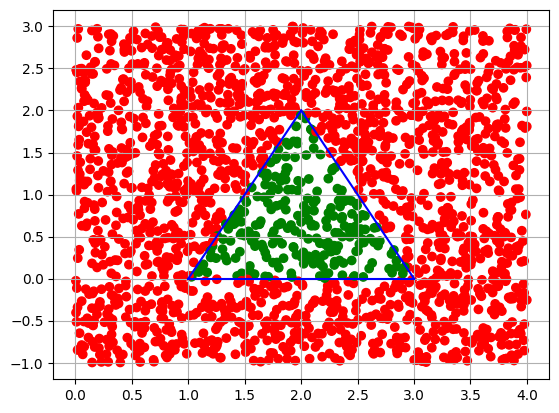
\includegraphics[width=0.8\textwidth]{1.png}
\caption{Visualization of classified 2D points using the McCulloch-Pitts neuron-based DFA. Green points are accepted, red points are rejected. Blue lines represent decision boundaries.}
\label{fig:dfa_plot}
\end{figure}

\section{Using Sigmoid Activation for Soft Classification}

In this variation, the activation function used by the McCulloch-Pitts neurons is changed from a binary \texttt{heavyside} function to a smooth \texttt{sigmoid} function. This transforms the system from a discrete logic gate simulator into a \textbf{soft classifier} that models probabilities.

\subsection*{Code Differences and Explanation}

\begin{minted}[fontsize=\small, bgcolor=gray!10, linenos]{python}
y = DFA(X, sigmoid)
c = np.where(y >= 0.5, 'green', 'red')
plt.scatter(X[0], X[1], c=c)
plt.plot([1, 2], [0, 2], c='b')
plt.plot([2, 3], [2, 0], c='b')
plt.plot([1, 3], [0, 0], c='b')
plt.grid(True)
plt.show()
\end{minted}

\subsection*{What Changed?}

\begin{itemize}
    \item The DFA model is now called with \texttt{sigmoid} as the activation function.
    \item Each neuron now returns a value in the range $[0, 1]$ instead of just 0 or 1.
    \item To turn these probabilities into binary decisions, we apply a threshold:
    \[
    \texttt{np.where}(y \geq 0.5, \text{'green'}, \text{'red'})
    \]
    \item This maintains consistency with the previous visualization (green for accepted, red for rejected), but now reflects a smoother decision surface.
\end{itemize}

\subsection*{Why Sigmoid?}

Using the sigmoid activation has the following effects:

\begin{enumerate}
    \item \textbf{Continuity:} The model can handle small variations in input smoothly.
    \item \textbf{Probabilistic output:} The final layer’s output can be interpreted as confidence in the classification.
    \item \textbf{Better visualization:} Especially useful when visualizing boundaries in a continuous space.
\end{enumerate}

\subsection*{Visual Output (Image 2)}

\begin{figure}[h!]
\centering
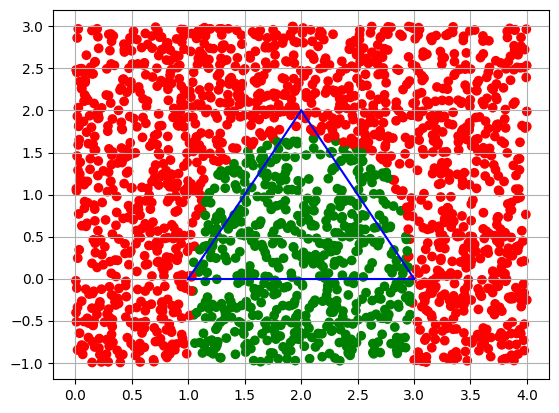
\includegraphics[width=0.8\textwidth]{2.png}
\caption{Soft classification using McCulloch-Pitts neurons with sigmoid activation. The boundary becomes smoother compared to the sharp Heaviside classifier.}
\label{fig:dfa_sigmoid_plot}
\end{figure}

\end{document}
